% !TEX root = Projektstudie.tex
% Steuerung

\section{Manuelle Steuerung}

\subsection{Joystick}
\begin{figure}
\centering
    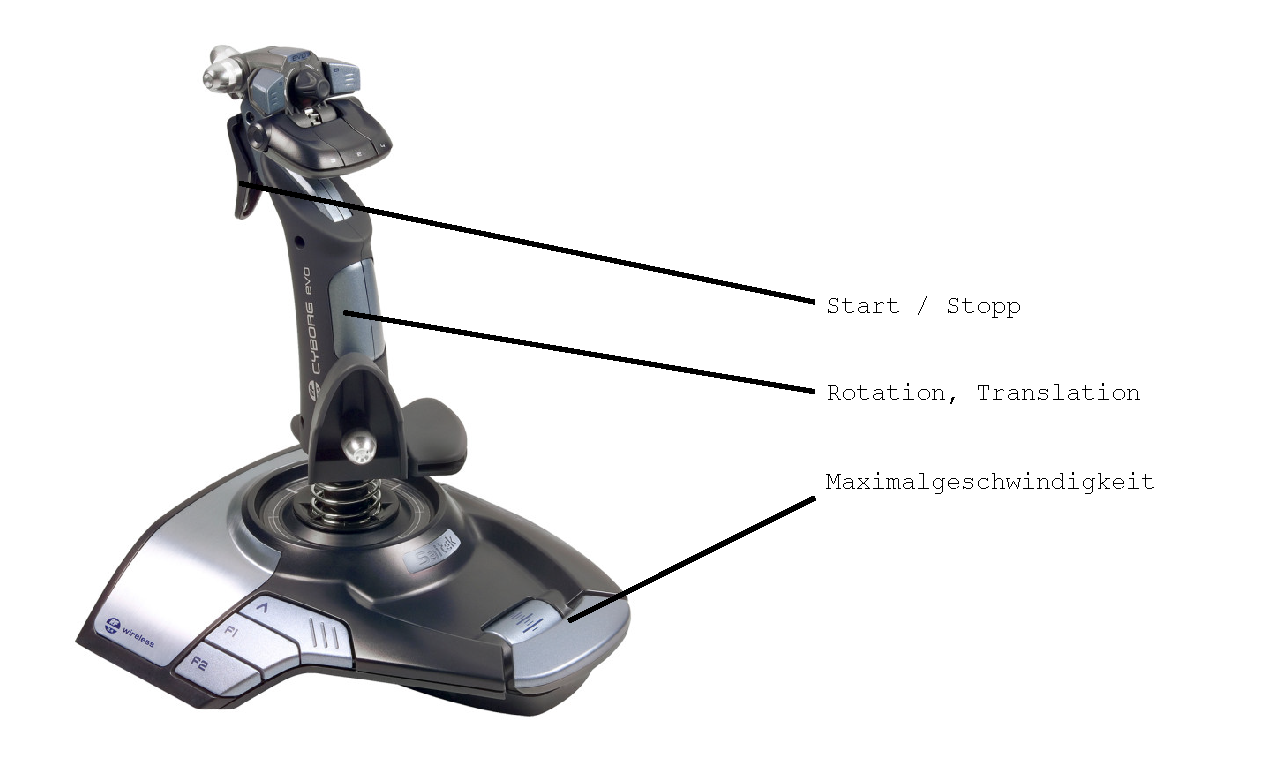
\includegraphics[width=.8\textwidth]{Abbildungen/Joystick}
    \caption[Funktionen des Joysticks]{Funktionen des Joysticks (Foto: www.saitek.de)}
    \label{fig:Joystick}
\end{figure}
Zur Steuerung des Mecanum-Roboters wird ein Joystick der Firma Saitek eingesetzt.
Dieser besitzt neben der x- und y- Achse auch einen rotatorischen Freiheitsgrad, mit dem die Drehbewegungen des Roboters gesteuert werden können.

Die Motoren werden durch das Drücken des Start/Stopp-Tasters mit dem Zeigefinger aktiviert. Aus Sicherheitsgründen muss der Taster für die Zeit der manuellen Steuerung gedrückt gehalten werden. Wird der Taster losgelassen, führt der Roboter einen Not-Stopp aus.

Zur Feinjustierung der Maximalgeschwindigkeit wird der in Abbildung~\ref{fig:Joystick} gezeigte Schubregler genutzt. Die aus der Rotations- und Translationsvorgabe resultierenden Radgeschwindigkeiten haben einen Wert $0 < v_i < 1$ und werden anschließend mit dem Wert des Schubreglers multipliziert, so dass maximal Geschwindigkeiten von 25000 Schritten pro Sekunde möglich sind.

\subsection{Visualisierung}
\begin{figure}
\centering
    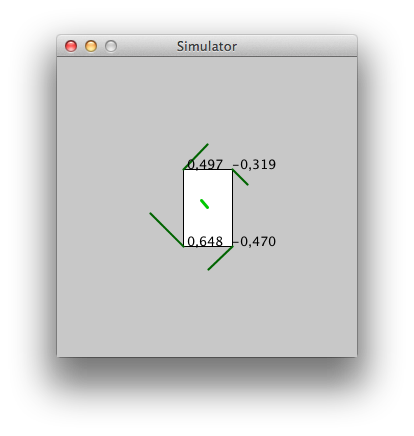
\includegraphics[width=.6\textwidth]{Abbildungen/Visualisierung}
    \caption[Visualisierung]{Screenshot des Steuerungsprogramms}
    \label{fig:Visualisierung}
\end{figure}
Vor der Programmierung des Roboters wird die Joystick-Eingabe und das mathematische Modell zunächst mit Hilfe einer Visualisierung validiert.
Die Visualisierung ist in der Programmiersprache Java\footnote{http://www.java.com} verfasst und ist damit plattformunabhängig.
Zur Vereinfachung der graphischen Ausgabe wird die \emph{Processing}\footnote{http://www.processing.org}-Library verwendet.
Der Joystick wird mit der Library \emph{proControll}\footnote{http://creativecomputing.cc/p5libs/procontroll} angesteuert.
Die Kommunikation mit dem Roboter findet mit den in Kapitel~\ref{sec:API} vorgestellten Befehlen über die serielle Schnittstelle statt. Die dazu notwendige Library \emph{Serial}\footnote{http://processing.org/reference/libraries/serial/} ist bereits Kern von Processing.
